\clearpage{}
\section{Region Typing}
\label{System:Regions}

% ---------------------
\subsection{Regions and aliasing}
A region is the set of store locations where a particular object may be present at runtime. We use regions to reason about the mutability and aliasing of objects. The following diagram shows a store containing a number of objects, divided into two regions. This diagram is intended to be suggestive only. Many systems besides our own make use of regions, and a particular system may allow them to be disjoint areas of the store, include free space, grow with time, be hierarchical, include only sub-components of an object, and so on.

\begin{center}
\includegraphics[scale=0.8]{2-System/fig/regions-inHeap}
\end{center}

We use $\rho_n$ to denote \emph{region handles}. A region handle can be thought of as a runtime identifier for a particular region, or perhaps an index into a table that describes the extent of a region. For the simple system in the diagram, we could treat a region as a set of aligned, 4-byte words. In this case our region handles could be defined as:


\code{
	$\rho_1$ & 	$ = \{ 1234, 1238, 1246, 1250 \}$ \\
	$\rho_2$ & 	$ = \{ 1682, 1690 \}$
}

At compile time we will not necessarily know how the objects in the store will be arranged, or how to define the region handles. We would like to write functions that operate on objects from any region, independently of how they are arranged. For this purpose we introduce \emph{region variables}, which we use to bind region handles. Region variables are identified as $r_n$ in this text.

There are conceptual similarities between region and value information. Consider the following statements of value:

\code{
	$23$ 	& $\mapsto \ < ... 10010 ... >$  \\
	$a$  	& $= 23$ \\
}

In the first statement, the numeral 23 represents an object in the store that includes a particular bit string. In the second statement we have used a \emph{value variable} to bind the numeral 23. We can think of regions as being akin to the objects in the store, region handles being akin to numerals, and region variables being like value variables. In this sense, regions are physical things, region handles are descriptions of them, and region variables are place holders for the handles.

Clearly though, regions and values are different kinds of things. As per tradition we use a star * to denote the kind of value types. Region kinds are denoted by a percent sign \%\footnote{Pictorially, \% is two circles separated by a line, a mnemonic for ``this, or that"}. In the concrete syntax we also use \% as a namespace qualifier, writing \texttt{\%rn} in place of $r_n$. This helps the parser, as well as being convenient for syntax highlighting text editors.

Unlike the system of Tofte and Birkedal \cite{tofte:region-inference}, ours deals only with region variables and not with the definition of region handles, or the layout of the store. Their system uses regions to manage the allocation of free space at run time, where ours uses regions as part of an analysis to guide compile time code optimisations.

Our analysis is type based. We add region variables to all type constructors which correspond to data objects that can be usefully updated. This includes constructors like $\iInt$, $\iBool$ and $\iList$, but not the function constructor $(\rightarrow)$ or the unit constructor $()$. The function constructor does not need one because the value of a function cannot be updated at runtime. The unit constructor does not need one because there is only one possible unit value.  

For example, a list of character pairs could have type:

\code{
 	$\ipairs$ & $:: \iList \ r_1 \ (\iPair \ r_2 \ (\iChar \ r_3) \ (\iChar \ r_4))$ \\
 	$\ipairs$ & $= [\iMkPair \ \texttt{'g'} \ \texttt{'o'}, \ \iMkPair \ \texttt{'b'} \ \texttt{'y'}, \ \dots ]$
}

In a top level signature such as this, if two type constructors have different region variables, such as $\iChar \ r_3$ and $\iChar \ r_4$, then the corresponding values are guaranteed to be represented by different run-time objects. However, in general these objects may \emph{alias}. For example, here is a function which creates a pair of integers:

\code{
	$\iintPair  :: \forall r_1 \ r_2 \ r_3. \ \iInt \ r_1 
			\to \iInt \ r_2 \to \iPair \ r_3 \ (\iInt \ r_1) \ (\iInt \ r_2)$ \\
 	$\iintPair  \ x \ y \ = \ \iMkPair \ x \ y$
}


As the region variables $r_1$, $r_2$ and $r_3$ are quantified in the type signature, we may pass the same integer object for both arguments of the function:

\code{
	$\ifive$ 	& $:: \iInt \ r_5$ 					\\
	$\ifive$ 	& $= 5$
}

\vspace{-1ex}
\code{
	$\ipairOfFives$	& $:: \iPair \ r_4 \ (\iInt \ r_5) \ (\iInt \ r_5)$ 	\\
	$\ipairOfFives$	& $= \iintPair \ \ifive \ \ifive$
}

Here, the region variables $r_1$ and $r_2$ of $\iintPair$ have been instantiated to $r_5$. This tells us that both elements of the pair may refer to the same heap object, and they will in this case. Note that in the body of $\iintPair$, the value variables $x$ and $y$ may also refer to the same object because we can pass the same one for both arguments.

In the type of $\ipairOfFives$, the region variable $r_4$ is fresh because the evaluation of $\iintPair$ will allocate a new object to represent the pair. Freshly allocated objects do not alias any existing objects.

Aliasing information is of fundamental importance when reasoning about destructive update, as any read or write actions performed on objects in one region will not be visible to the parts of a program that only deal with another. To use the language of \cite{reynolds:interference}, actions performed on disjoint regions do not \emph{interfere}.

In many cases the region variables attached to differently named type constructors will be distinct, but this is not required in general. In our $\ipairs$ example, all the list constructor cells are in one region, and all the pair cells are in another:

\smallskip
\begin{center}
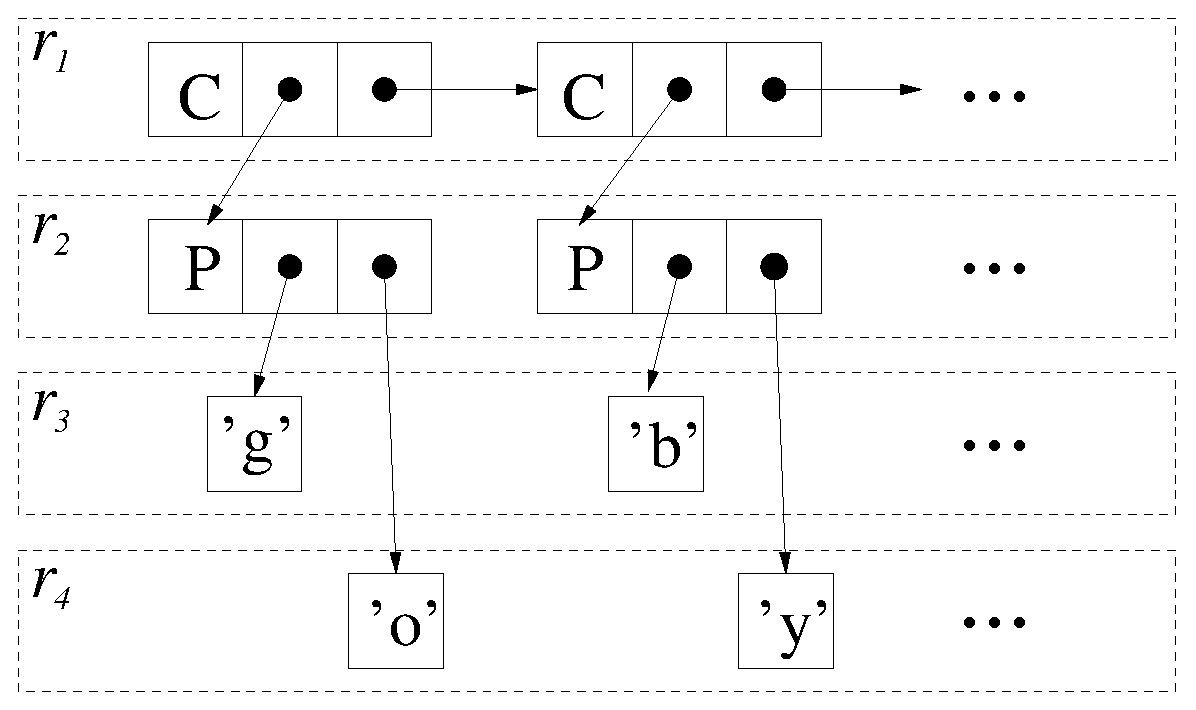
\includegraphics[scale=0.4]{2-System/fig/regions-list.eps}
\end{center}
\smallskip

Setting $r_1 = r_2$ would be equivalent to placing the list cells in the same region as the pair cells. 

Like Talpin and Jouvelot's original work \cite{talpin:discipline}, our concept of a region is simply a name for a set of locations. We sometimes find it useful to visualise regions as colours of paint, which we apply to data objects stored in the heap. Setting $r_1 = r_2$ corresponds to painting all the list and pair cells the same colour. They will be harder to distinguish afterwards, corresponding to a weakening of our analysis, but it will cause them no harm.

As region variables are provided as parameters to type constructors, the kinds of the constructors reflect this. $\iChar$ takes a region and produces a type. $\iList$ takes a region, a type, and produces a new type. $\iPair$ takes a region, two types, and produces a new type:

\code{
	$\iChar$ 	& $:: \% \to *$ \\
	$\iList$ 	& $:: \% \to * \to *$ \\
	$\iPair$ 	& $:: \% \to * \to * \to *$ 
}


% ---------------------------
\subsection{Region classes}
When a value is mutable we add mutability constraints to the region variables in its type. For example, if we wanted to update the characters in a string we would give it type:

\code{
 	$\istr :: \iMutable \ r_2 \Rightarrow \iList \ r_1 \ (\iChar \ r_2)$
}

The constraint $\iMutable \ r_2$ is a \emph{region class}. Region classes are similar to the value type classes in Haskell \cite{hall:type-classes}, such as $Show$ and $Eq$. With value type classes, the type constraint $Eq \ a$ requires $a$ to be a type that supports equality. Similarly, the region constraint $\iMutable \ r_2$ requires $r_2$ to correspond with a region that supports update.

When discussing our system we use the word ``type'' to refer to all the information in a signature, including value type information such as $\iList$ and $\iChar$, any constraints on variables, region information, as well as the effect and closure information we will discuss later. For this reason we also refer to both region classes and value type classes as simply ``type classes". Note that the programmer usually doesn't have to provide this additional information in type signatures. Most can be reconstructed by the type inferencer. This is discussed further in \S\ref{System:Projections:ambiguous} and \S\ref{Inference:Generalisation:late-constraints}.

Returning to the signature of $\istr$, we call term on the right of the $\Rightarrow$, the \emph{body} of the type. We call the value portion of the body is its \emph{shape}, because this information describes the overall structure of the object in the store.

As our types often contain a large number of constraints, we usually write them after the body, instead of before it as in Haskell:

\code{
	$\istr$ 
	& $::$		& $\iList \ r_1 \ (\iChar \ r_2)$ \\
    	& $\rhd$	& $\iMutable \ r_2$
}

The $\rhd$ is pronounced ``with'', and is written as \texttt{:-} in the concrete syntax. The difference between the above type and the original prefix form is purely syntactic, and our compiler accepts both.

In the above type, no constraint has been placed on $r_1$. If we wish to update the spine of the list as well as its characters, then this region must also be mutable. Multiple constraints are separated by commas:

\code{
	$\istr$ 
	& $::$		& $\iList \ r_1 \ (\iChar \ r_2)$ \\
    	& $\rhd$	& $\iMutable \ r_1$ \\
	& $,$		& $\iMutable \ r_2$
}

Being able to update the spine of a list is useful for operations such as inserting a new element into the middle of the list, as it allows us to change the tail pointers of existing cons cells.

On the other hand, if we wish to \emph{prevent} updates to the spine we could use the constraint $\iConst \ r_1$ to enforce this:

\code{
	$\istr$ 
	& $::$		& $\iList \ r_1 \ (\iChar \ r_2)$ \\
    	& $\rhd$	& $\iConst \ r_1$ \\
	& $,$		& $\iMutable \ r_2$
}

As there are two region variables in this type, both the spine and elements can have differing mutabilities. Attempting to constrain a region variable to be both $\iMutable$ and $\iConst$ results in a compile time type error. 


% ---------------------
\subsection{Functions, allocation and non-material regions}
\label{System:Regions:non-material}
In our system the successor function has the following signature:


\code{
 	$\isucc :: \forall (r_1 :: \%) \ (r_2 :: \%). \ \iInt \ r_1 \to \iInt \ r_2$
}

In this type we have included the kind of each region variable, but as in Haskell we can omit this information if it can be easily inferred. The variables $r_1$ and $r_2$ must have region kind because they are used as parameters to the $\iInt$ constructor, so we instead write:

\code{
 	$\isucc :: \forall r_1 \ r_2. \ \iInt \ r_1 \to \iInt \ r_2$
}

Starting with the $\iInt \ r_1$ term on the left of the arrow, the fact that $r_1$ is quantified indicates that $\isucc$ can operate on values from any region. On the right of the arrow, the fact that $r_2$ is quantified indicates that $\isucc$ can produce its output \emph{into} any region. This is possible because the function allocates a new $\iInt$ object each time it is called, and freshly allocated objects do not alias existing objects. Alternatively, if a function does not allocate its return value, then the region variables in its return type will not be quantified:

\code{
	& $x :: \iInt \ r_3$ \\
	& $x = 5$ 
	\\[1ex]
	& $\isameX :: () \to \iInt \ r_3$ \\
	& $\isameX \ () = x$ \\
}

In this example, $\isameX$ returns the same object every time it is called. This object comes from its environment, and is shared between all calls to it, hence $r_3$ must remain unquantified. Unquantified region variables can also appear on the left of an arrow. This happens when a function conflates its arguments with values from the environment:

\code{
	& $y :: \iInt \ r_4$ \\
	& $y = 23$ 
	\\[1ex]
	& $\ichooseY :: \iInt \ r_4 \to \iInt \ r_4$ \\
	& $\ichooseY z = \kif \ ... \ \kthen \ y \ \kelse \ z$ \\
}

The object returned by $\ichooseY$ could be either its argument $z$, or the shared object $y$. Our system cannot represent the fact that the returned object might be in one region \emph{or} another, so we use the same variable for both. This limitation is discussed in \S\ref{Evaluation:Limitations:blocked-regions}. In this example, $r_4$ is also present in the environment, so it cannot be quantified in the type of $\ichooseY$. 

Although $r_4$ appears in the types of both $y$ and $\ichooseY$, each occurrence has a slightly different meaning. In the type of $y$, it represents a particular set of locations in the heap, and one of those locations contains the integer object of value 23. On the other hand, the use of $r_4$ in the type of $\ichooseY$ does not mean that $\ichooseY$ also contains an integer object. Instead, these occurrences represent locations in the store where the function's argument and return values lie. We distinguish between these two cases by saying that $r_4$ in the type of $y$ is in a \emph{material} position, whereas in the type of $\ichooseY$ is not. The difference between the material and immaterial positions of type constructors is discussed more fully in \S\ref{System:Closure:non-material-regions}.


% ---------------------
\subsection{Updating data requires it to be mutable}
\label{System:Regions:update}
When a function can update its argument, we add a constraint to its type that requires the argument to be mutable. For example, the $inc$ function destructively increments its argument and has type:

\code{
	$\iinc$ 	
	& $::$		& $\forall r_1. \ \iInt \ r_1 \to ()$ \\
    	& $\rhd$	& $\iMutable \ r_1$ \\
}

This type indicates that $\iinc$ can operate on integers in any region, as long as that region is mutable. We treat mutability as a capability provided by the objects in our system, and the requirement for this capability flows from the functions that make use of it. An alternative setup would be to explicitly \emph{permit} update by requiring the programmer to supply type signatures and mutability constraints for every object that is to be updated, or to use a special keyword when allocating them. We feel that the use of a special keyword would create clutter in the program, though we will sometimes require mutability constraints to be given in a type signature. We will return to this in \S\ref{Inference:Generalisation:late-constraints}.

During type inference, the compiler compares all the constraints placed on the region variables in the program. In the absence of an explicit type signature, if a particular region is not constrained to be mutable, then at runtime the objects contained within that region will never be passed to a function that can update them. For this reason, material region variables that are not constrained to be mutable are considered to be constant.

This does not apply to quantified, immaterial regions in the types of functions. In this case the three options: mutable, constant, and unconstrained, have distinct meanings. For example, in the following type signature:

\code{
 	$\ifoo :: \forall r_1. \ \iInt \ r_1 \to ()$
}

As $r_1$ is unconstrained we may apply this function to integers which are either mutable or constant, whereas with:

\code{
 	$\ifoo'$
	& $::$		& $\forall r_1. \ \iInt \ r_1 \to ()$ \\
	& $\rhd$	& $\iConst \ r_1$
}

We can only apply this function to integers which are constant.


% ---------------------
\subsection{Primary regions and algebraic data}
In all examples so far, the type constructors used have had only one region parameter. This is typical for simple types with a small amount of internal structure, but we need more when defining algebraic data. Consider a vector of two integers:

\code{
	\mc{2}{$\kdata \ \iIntVector \ r_1 \ r_2 \ r_3$} \\
	& $= \iIV \ (\iInt \ r_2) \ (\iInt \ r_3)$
}

The first region variable $r_1$ corresponds to the region containing the outer $\iIV$ constructor. This is called the \emph{primary region variable}. The variables $r_2$ and $r_3$ appear in the body of the definition and represent the regions containing the integer components. For example, the value $(\iIV \ 2 \ 3)$ would be represented as:

\smallskip
\begin{center}
\includegraphics[scale=0.5]{2-System/fig/regions-intVector.eps}
\end{center}

These three separate region variables provide three degrees of freedom when deciding which parts of the object should be mutable and which should be constant. Allowing $r_2$ and/or $r_3$ to be mutable permits the components to be updated, and when $r_1$ is mutable we can update the pointers in the outer constructor. The \emph{tag} of the outer constructor is also contained in the primary region. Updates to the tag permit the value of enumerations such as $\iBool$ to be changed. 

Note that with this system it is not possible to give the \emph{pointers} to the two components separate region variables. We omit this capability to reduce the complexity of the system, though we see no fundamental barrier to supporting it if required in the future.



% --------------------
\subsection{Thinking about regions}
There are several ways to conceptualise what a region actually ``is'', and we have mentioned two so far. Firstly, a region is an area of the heap where objects can be stored at runtime. For systems that use regions to manage allocation and deallocation \cite{tofte:mlkit-4.3.0}, this is the most natural. Fresh objects are allocated into a particular region, and the whole region is reclaimed by the storage manager when the objects contained are no longer needed by the running program. Such systems use region allocation to augment or replace the standard garbage collection mechanism. At an operational level, the regions in such systems are usually contiguous, or are constructed with a linked list of contiguous memory pages. However, DDC does not use regions to manage allocation, it relies on a traditional garbage collector. We can still imagine a region to be a specific area of the heap, but the parts of the heap that make up the region are scattered throughout, and do not form a contiguous block.

Secondly, a region is a label for a collection of objects in the store. Earlier we suggested imagining these labels to be like colours of paint. When a program is compiled, the compiler decides on a fixed set of colours (regions). It then pretends that at runtime, every object allocated by the program will be painted with one of these colours. The colours help it to reason about what the program is permitted to do with a certain object. For example, we could paint all the mutable objects with shades of pink, and all the constant objects with shades of blue. Importantly though, the colours are just pretend. Our analysis is static, so we do not record what region an object belongs to in the object itself, or maintain any region information at runtime.

Finally, a region is a label for a set of program points which perform allocation \cite{pierce:atapl}. If we know that a particular object is in region $r_1$, then it must have been allocated by one of the points corresponding to $r_1$. Every object is allocated by one program point, and an allocation point can allocate zero or more objects. Allocation points exist within functions, so whether or not an allocation point ever allocates depends on whether the function is ever called. However, during evaluation the objects tend to get mixed up, such as when choosing between two objects in an if-expression. This means that the compiler will usually lose track of the exact point where a particular object was allocated. It can only hope to reduce it to a small set of possibilities.  Using this idea we can imagine that if a region variable is constrained to be $\iConst$, some part of the program requires an allocation point to produce a constant object. Likewise, if a region variable is constrained to be $\iMutable$, some part of the program requires a mutable object. A mutability conflict arises when a particular allocation point must produce an object that is both mutable and constant. This is not possible, so we report an error. We will exploit this line of reasoning further when we come to prove the soundness of our core language in \S\ref{Core:Language:Soundness}.


